% Asset ID: A21FunctionsAndGraphsTIKZ-007
% Unit: A21: A2 1 Pure Mathematics
% Topic code: A21-AF
% Related LO IDs: A21-AF-LO006, A21-AF-LO007
% Related lesson section: y = |f(x)| and y = f(|x|)
% Source: Chapter 2 Functions and Graphs transformed modulus section
% Purpose: Compare outside modulus and inside modulus transformations.

\documentclass[tikz,border=8pt]{standalone}
\usepackage{amsmath}
\begin{document}
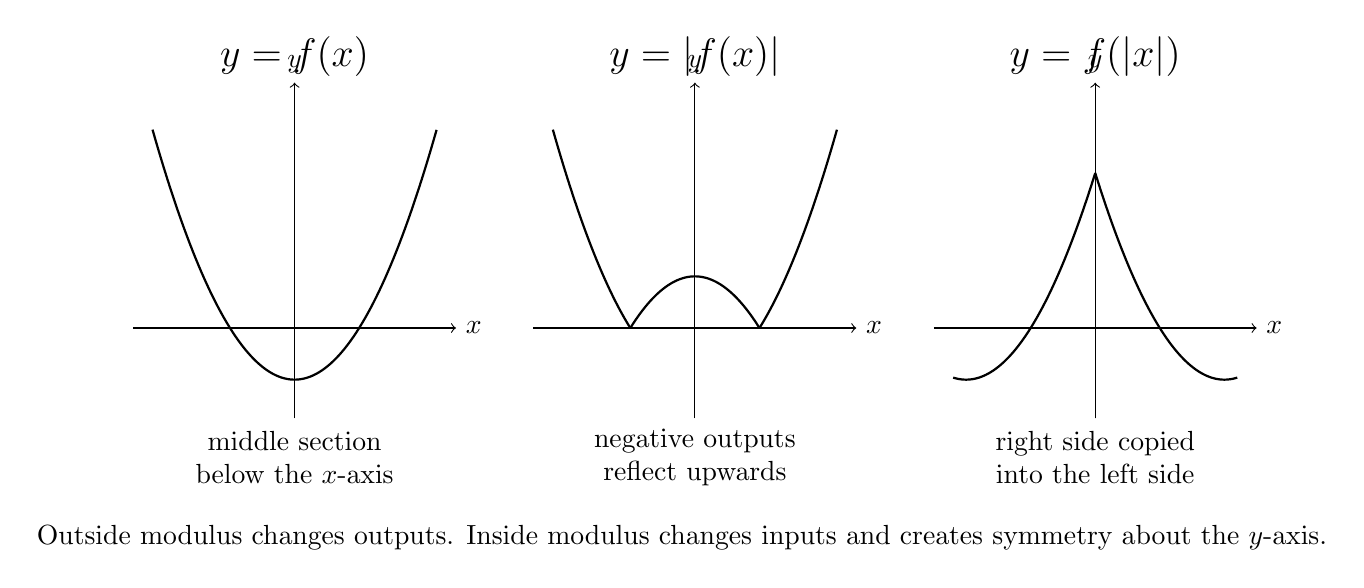
\begin{tikzpicture}[scale=0.82]
\begin{scope}[shift={(0,0)}]
\node at (2,4.2) {\Large $y=f(x)$};
\draw[->] (-0.5,0) -- (4.5,0) node[right] {$x$};\draw[->] (2,-1.4) -- (2,3.8) node[above] {$y$};
\draw[thick, domain=-0.2:4.2, samples=100] plot (\x,{0.8*(\x-1)*(\x-3)});
\node[align=center] at (2,-2.0) {middle section\\below the $x$-axis};
\end{scope}
\begin{scope}[shift={(6.2,0)}]
\node at (2,4.2) {\Large $y=|f(x)|$};
\draw[->] (-0.5,0) -- (4.5,0) node[right] {$x$};\draw[->] (2,-1.4) -- (2,3.8) node[above] {$y$};
\draw[thick, domain=-0.2:1, samples=40] plot (\x,{0.8*(\x-1)*(\x-3)});
\draw[thick, domain=1:3, samples=60] plot (\x,{-0.8*(\x-1)*(\x-3)});
\draw[thick, domain=3:4.2, samples=40] plot (\x,{0.8*(\x-1)*(\x-3)});
\node[align=center] at (2,-2.0) {negative outputs\\reflect upwards};
\end{scope}
\begin{scope}[shift={(12.4,0)}]
\node at (2,4.2) {\Large $y=f(|x|)$};
\draw[->] (-0.5,0) -- (4.5,0) node[right] {$x$};\draw[->] (2,-1.4) -- (2,3.8) node[above] {$y$};
\draw[thick, domain=2:4.2, samples=80] plot (\x,{0.8*((\x-2)-1)*((\x-2)-3)});
\draw[thick, domain=-0.2:2, samples=80] plot (\x,{0.8*((2-\x)-1)*((2-\x)-3)});
\draw[dashed] (2,-1.4) -- (2,3.8);
\node[align=center] at (2,-2.0) {right side copied\\into the left side};
\end{scope}
\node[align=center] at (8,-3.25) {Outside modulus changes outputs. Inside modulus changes inputs and creates symmetry about the $y$-axis.};
\end{tikzpicture}
\end{document}
